\documentclass[11pt,oneside,openany]{book}

\usepackage[a4paper,margin=24mm,headheight=15pt]{geometry}
\usepackage{graphicx}
\usepackage{booktabs}
\usepackage{longtable}
\usepackage{array}
\usepackage{tabularx}
\usepackage{amsmath,amssymb}
\usepackage{siunitx}
\usepackage{xcolor}
\usepackage{microtype}
\usepackage{listings}
\usepackage{enumitem}
\usepackage{fancyhdr}
\usepackage{caption}
\usepackage{subcaption}
\usepackage{tikz}
\usetikzlibrary{arrows.meta,positioning,shapes.geometric,fit,backgrounds,calc}
\usepackage[hidelinks]{hyperref}
\usepackage{bookmark}

\definecolor{MigaNavy}{HTML}{24394D}
\definecolor{MigaBlue}{HTML}{0D6EFD}
\definecolor{MigaCyan}{HTML}{00A6C7}
\definecolor{MigaGreen}{HTML}{198754}
\definecolor{MigaGold}{HTML}{D79B00}
\definecolor{MigaRed}{HTML}{B83232}
\definecolor{MigaLight}{HTML}{F2F5F8}
\definecolor{MigaGray}{HTML}{5B6472}

\hypersetup{
  pdftitle={MIGA Controller: Operation, Optimization and Analysis Manual},
  pdfauthor={Yiming MENG},
  pdfsubject={MIGA Controller marker-optimization branch},
  colorlinks=true,
  linkcolor=MigaBlue,
  urlcolor=MigaCyan,
  citecolor=MigaGreen
}

\graphicspath{{assets/}}
\setcounter{tocdepth}{2}
\setcounter{secnumdepth}{3}
\setlist{nosep,leftmargin=1.6em}
\renewcommand{\arraystretch}{1.18}

\pagestyle{fancy}
\fancyhf{}
\fancyhead[L]{\small\textcolor{MigaGray}{MIGA Controller Manual}}
\fancyhead[R]{\small\textcolor{MigaGray}{\leftmark}}
\fancyfoot[C]{\thepage}
\renewcommand{\headrulewidth}{0.3pt}

\lstdefinestyle{miga}{
  basicstyle=\ttfamily\small,
  keywordstyle=\color{MigaBlue}\bfseries,
  commentstyle=\color{MigaGreen},
  stringstyle=\color{MigaRed},
  backgroundcolor=\color{MigaLight},
  frame=single,
  rulecolor=\color{MigaGray!35},
  breaklines=true,
  columns=fullflexible,
  keepspaces=true,
  showstringspaces=false
}
\lstset{style=miga}

\tikzset{
  block/.style={draw=MigaNavy,rounded corners=2pt,fill=MigaLight,align=center,
    minimum height=9mm,text width=27mm,font=\small},
  primary/.style={block,fill=MigaBlue!10,draw=MigaBlue},
  analysis/.style={block,fill=MigaGold!12,draw=MigaGold},
  store/.style={block,fill=MigaGreen!10,draw=MigaGreen},
  warning/.style={block,fill=MigaRed!8,draw=MigaRed},
  flow/.style={-{Latex[length=2mm]},thick,draw=MigaNavy},
  feedback/.style={-{Latex[length=2mm]},thick,dashed,draw=MigaRed}
}

\newcommand{\code}[1]{\texttt{\detokenize{#1}}}
\newcommand{\ui}[1]{\textbf{#1}}
\newcommand{\pathcode}[1]{\nolinkurl{#1}}
\newcommand{\branchname}{\texttt{marker-optimization}}
\newcommand{\commitid}{\texttt{f60eef0}}
\newcommand{\warningtext}[1]{\par\medskip\noindent
  \fcolorbox{MigaRed}{MigaRed!5}{\parbox{0.93\linewidth}{\textbf{Caution.} #1}}\par\medskip}
\newcommand{\notetext}[1]{\par\medskip\noindent
  \fcolorbox{MigaBlue}{MigaBlue!5}{\parbox{0.93\linewidth}{\textbf{Note.} #1}}\par\medskip}
\newenvironment{procedure}[1]
  {\par\medskip\noindent\textbf{Operating procedure: #1}\par\smallskip\begin{enumerate}}
  {\end{enumerate}\medskip}

\begin{document}

\begin{titlepage}
  \thispagestyle{empty}
  \centering

  \vspace*{13mm}
  {\large\scshape MIGA Project\par}
  \vspace{2mm}
  {\normalsize Cold Atoms Bordeaux\par}

  \vspace{22mm}
  {\color{MigaNavy}\rule{0.78\textwidth}{0.8pt}\par}
  \vspace{12mm}

  {\color{MigaNavy}\bfseries\fontsize{31}{37}\selectfont
    MIGA Controller\par}
  \vspace{8mm}
  {\Large Operation, Optimization and Analysis\par}
  \vspace{3mm}
  {\Large Manual\par}

  \vspace{12mm}
  {\color{MigaNavy}\rule{0.78\textwidth}{0.8pt}\par}
  \vspace{10mm}
  {\large\scshape Technical Reference Manual\par}
  \vspace{3mm}
  {\normalsize Complete reference for the \branchname{} branch\par}

  \vfill

  \begin{tabular}{>{\raggedleft\arraybackslash}p{34mm} p{64mm}}
    \textit{Prepared by} & Yiming MENG\\[3mm]
    \textit{Project} & MIGA / Cold Atoms Bordeaux\\[3mm]
    \textit{Source revision} & \commitid\\[3mm]
    \textit{Document date} & \today
  \end{tabular}

  \vfill

  \begin{minipage}{0.78\textwidth}
    \centering
    \small\color{MigaGray}
    Laboratory control software for cold-atom acquisition, sequence generation,
    synchronized measurements, online optimization and reproducible archive analysis.
  \end{minipage}

  \vspace{9mm}
  {\color{MigaNavy!45}\rule{0.42\textwidth}{0.45pt}\par}
  \vspace*{5mm}
\end{titlepage}
\color{black}

\frontmatter
\chapter*{Document status and scope}
\addcontentsline{toc}{chapter}{Document status and scope}
This manual describes the behavior implemented in the local \branchname{} checkout at
revision \commitid. It is written for experimental operators, analysts and maintainers.
The graphical user interface, backend routes, data models, numerical routines and tests
were reviewed together; therefore a feature is documented only when an executable code
path or test supports it. Values shown in screenshots are examples and are not universal
experimental calibrations.

\warningtext{The controller can compile pulse sequences, trigger laboratory hardware and
write DDS tables. Confirm beam states, trigger routing, voltage limits and emergency stop
procedures before leaving simulation mode. Never treat a successful web request as proof
that the optical or electronic apparatus is safe.}

\section*{How to use this manual}
Operators should begin with Chapters~\ref{ch:install}, \ref{ch:console} and
\ref{ch:trouble}. Users creating parameterized sequences should then read
Chapters~\ref{ch:sequence} and \ref{ch:markers}. Optimization users should read
Chapters~\ref{ch:markeropt} and \ref{ch:bayes}. Analysts should concentrate on
Chapters~\ref{ch:signal}, \ref{ch:archive} and \ref{ch:stability}. Maintainers can use
the architecture, API and source-map appendices as an implementation index.

\tableofcontents
\listoffigures
\listoftables

\mainmatter

\chapter{System overview}\label{ch:overview}

\section{Purpose}
MIGA Controller is a browser-based control and data-acquisition application for cold-atom
experiments. It combines sequence parameterization, compilation, hardware triggering,
dual-channel acquisition, fit-based and integration-based analysis, live visualization,
archiving and offline re-analysis. The \branchname{} branch adds two complementary
closed-loop workflows: deterministic sequential marker optimization and Ax-based Bayesian
optimization. It also includes synchronized master/slave scans, scheduled runs, AC Stark
and lock-in modes, Bragg pulse generation, Bragg phase-space analysis, archive collections
and overlapping Allan deviation.

\section{Functional map}
\begin{figure}[htbp]
\centering
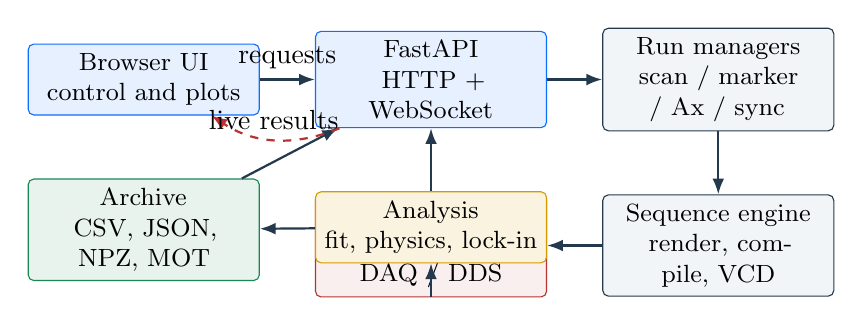
\begin{tikzpicture}[node distance=8mm and 7mm]
  \node[primary] (ui) {Browser UI\\control and plots};
  \node[primary,right=of ui] (api) {FastAPI\\HTTP + WebSocket};
  \node[block,right=of api] (mgr) {Run managers\\scan / marker / Ax / sync};
  \node[block,below=of mgr] (seq) {Sequence engine\\render, compile, VCD};
  \node[warning,left=of seq] (hw) {Hardware\\Red Pitaya / DAQ / DDS};
  \node[analysis,below=of api] (math) {Analysis\\fit, physics, lock-in};
  \node[store,below=of ui] (data) {Archive\\CSV, JSON, NPZ, MOT};
  \draw[flow] (ui)--node[above]{requests}(api);
  \draw[flow] (api)--(mgr);
  \draw[flow] (mgr)--(seq);
  \draw[flow] (seq)--(hw);
  \draw[flow] (hw)--(math);
  \draw[flow] (math)--(data);
  \draw[flow] (math)--(api);
  \draw[flow] (data)--(api);
  \draw[feedback] (api) to[bend left=28] node[above]{live results}(ui);
\end{tikzpicture}
\caption{End-to-end control and analysis architecture. The WebSocket path returns shot
results without blocking the acquisition worker.}
\label{fig:architecture}
\end{figure}

\section{User-facing applications}
\begin{table}[htbp]
\centering
\caption{Primary browser interfaces.}
\begin{tabularx}{\textwidth}{>{\bfseries}l l X}
\toprule
Page & Path & Purpose\\
\midrule
Control Console & \pathcode{/index.html} & Immediate, scheduled and synchronized scans;
live fit and waveform plots; sequence upload and scan export.\\
Marker Workflow & \pathcode{/marker-optimize.html} & Ordered, fail-fast optimization of
named sequence markers.\\
Optimization & \pathcode{/optimize.html} & Ax-based online search across discrete
\code{PARAMETER} variables.\\
Data Archive & \pathcode{/archive.html} & Run browsing, collections, waveform inspection,
recalculation, scan fitting, Allan and Bragg phase analysis.\\
Settings & \pathcode{/settings.html} & Hardware, physics, calibration, marker, fit, sync,
path and update configuration.\\
\bottomrule
\end{tabularx}
\end{table}

\section{Recommended operating sequence}
\begin{enumerate}
  \item Verify paths, hardware platform, network endpoints and analysis constants.
  \item Load a sequence and preview the parameterized output.
  \item Perform a short simulation scan and inspect both waveform channels.
  \item Switch to real hardware only after the trigger and voltage limits are verified.
  \item Label the run, execute it, and confirm that its archive contains configuration,
  results, sequence snapshot and waveform files.
  \item Use an optimization workflow only after a bounded manual scan shows that the
  objective metric is valid over the proposed search interval.
\end{enumerate}

\chapter{Installation and startup}\label{ch:install}

\section{Requirements}
The backend requires Python and the packages listed in \pathcode{requirements.txt}.
Real operation additionally requires the local sequence toolchain (normally
\code{tmot4} and \code{cmot4}), access to the selected acquisition platform, and any
site-specific DDS writer used for AC Stark operation. Bayesian optimization requires
\code{ax-platform}. Browser assets are currently loaded from CDNs, so an offline
installation must provide cached or locally vendored Vue, Axios, Plotly and Bootstrap
assets.

\section{Launcher}
The preferred entry point is:
\begin{lstlisting}[language=bash]
./launch_code
\end{lstlisting}
The graphical launcher creates \pathcode{.venv/} when required, checks packages,
validates the Ax import path, exposes the \code{tmot4}/\code{cmot4} path status, starts
or stops the backend and displays the server log. Without a graphical desktop it falls
back to the terminal launcher.

\begin{table}[htbp]
\centering
\caption{Terminal launcher commands.}
\begin{tabularx}{\textwidth}{l X}
\toprule
Command & Effect\\
\midrule
\code{./start_controller.sh} & Interactive start using the project virtual environment.\\
\code{./start_controller.sh --check-only} & Validate the environment without starting.\\
\code{./start_controller.sh --status} & Report launcher and server state.\\
\code{./start_controller.sh --start-detached} & Start in the background.\\
\code{./start_controller.sh --stop} & Request a controlled server stop.\\
\bottomrule
\end{tabularx}
\end{table}

\section{First-time configuration}
Open \url{http://127.0.0.1:8000/settings.html}. In \ui{System Paths}, select the
\code{mot4ztex} directory or enter explicit compiler and template paths. In
\ui{Network}, choose Red Pitaya or local DAQ and set a timeout longer than the longest
expected device response. In \ui{Physics \& Gains}, set gains, signal thresholds and
calibration constants. Finally, start in simulation mode and run a minimal scan.

\begin{procedure}{first-start verification}
  \item Run \code{./start_controller.sh --check-only} and resolve every missing path.
  \item Open the Control Console and confirm the status is \ui{IDLE}.
  \item Load the default sequence and check that a preview can be generated.
  \item Use a two-point simulation scan and verify that the WebSocket terminal reports
  both acquisition and analysis completion.
  \item Open the archive and confirm that the new run is readable.
\end{procedure}

\chapter{Architecture and execution pipeline}\label{ch:architecture}

\section{Application layers}
\pathcode{main.py} creates the FastAPI application, installs CORS, registers the API
router, defines \pathcode{/ws}, and mounts the static frontend last so that it cannot
intercept WebSocket requests. The singleton \code{ExperimentManager} executes blocking
hardware work in background threads. A thread-safe bridge submits result broadcasts to
the main asynchronous event loop.

Pydantic models in \pathcode{app/models/schemas.py} validate incoming configurations.
Core managers build scan plans, enforce an exclusive run slot, operate hardware and
write archives. Analysis modules contain numerical logic without UI state. This
separation allows the archive to re-run calculations against stored waveforms.

\section{Shot lifecycle}
\begin{figure}[htbp]
\centering
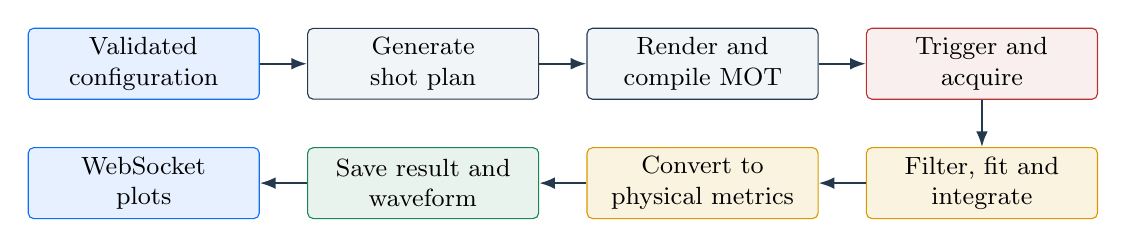
\begin{tikzpicture}[node distance=6mm]
  \node[primary] (cfg) {Validated\\configuration};
  \node[block,right=of cfg] (plan) {Generate\\shot plan};
  \node[block,right=of plan] (render) {Render and\\compile MOT};
  \node[warning,right=of render] (trigger) {Trigger and\\acquire};
  \node[analysis,below=of trigger] (fit) {Filter, fit and\\integrate};
  \node[analysis,left=of fit] (phys) {Convert to\\physical metrics};
  \node[store,left=of phys] (save) {Save result and\\waveform};
  \node[primary,left=of save] (stream) {WebSocket\\plots};
  \draw[flow] (cfg)--(plan);
  \draw[flow] (plan)--(render);
  \draw[flow] (render)--(trigger);
  \draw[flow] (trigger)--(fit);
  \draw[flow] (fit)--(phys);
  \draw[flow] (phys)--(save);
  \draw[flow] (save)--(stream);
\end{tikzpicture}
\caption{Per-shot execution. A failed shot emits an error payload and does not silently
become a numeric data point.}
\label{fig:shot-life}
\end{figure}

\section{Exclusive run ownership}
Standard scans, schedules, marker optimization, Bayesian optimization and synchronized
runs share the same experiment hardware. The manager therefore exposes a run slot with
an active-mode label. A second workflow is rejected while that slot is owned. Stop
requests set workflow-specific flags and then release the slot only after the worker has
closed its archive and restored any temporary hardware state.

\section{Timing from VCD}
The sequence compiler produces a VCD representation. \code{VCDParser} locates the
configured launch and trigger channels and determines their physical time separation.
This delay enters arrival-time and time-of-flight interpretation. A missing channel is a
configuration or sequence error; it should not be replaced with an assumed delay.

\chapter{Sequence files and parameterization}\label{ch:sequence}

\section{Classic placeholders}
Classic mode replaces \code{PARAMETER0}, \code{PARAMETER1} and \code{PARAMETER2} in the
active \code{.mot} template. Each axis can be floating-point or integer. Integer values
are rounded at the boundary where the scan plan is built; floating-point values are
rounded to six decimal places.

For a step-size axis, the sign of the user step is ignored and the direction follows the
relative order of start and stop. The stop point is included when it lies on the grid,
within a floating-point tolerance. For an $N$-point axis, values are linearly spaced:
\begin{equation}
  p_i=p_{\min}+\frac{i}{N-1}(p_{\max}-p_{\min}),\qquad i=0,\ldots,N-1.
\end{equation}
An explicit comma-separated list preserves the specified order after numeric validation.

\section{Multidimensional scans}
Two- and three-dimensional scans use the Cartesian product of the independent axes:
\begin{equation}
  \mathcal{P}=\mathcal{P}_0\times\mathcal{P}_1\times\mathcal{P}_2.
\end{equation}
Only Standard mode is permitted for multidimensional scans. Each complete grid is
repeated according to \ui{Averages}; if \ui{Randomize} is enabled, the expanded shot
list is shuffled.

\begin{figure}[htbp]
\centering
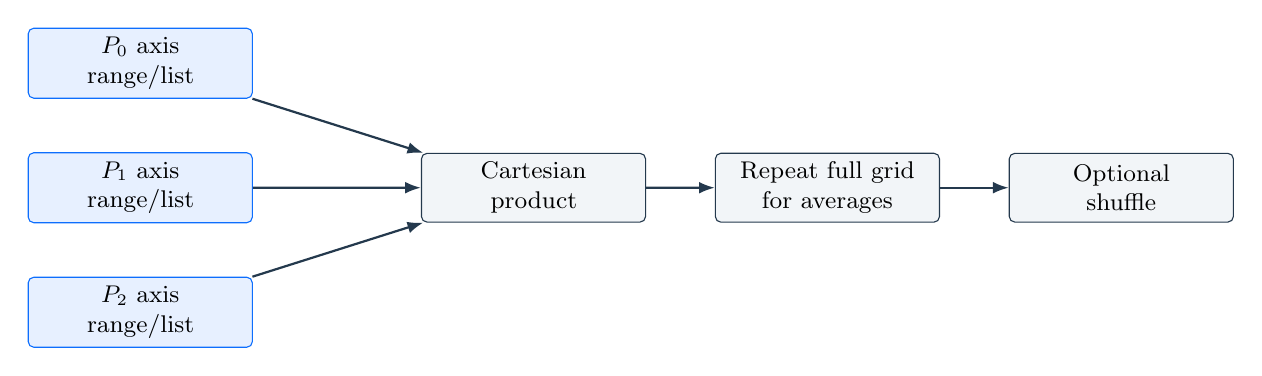
\begin{tikzpicture}[node distance=7mm and 9mm,scale=0.97,transform shape]
  \node[primary] (a0) {$P_0$ axis\\range/list};
  \node[primary,below=of a0] (a1) {$P_1$ axis\\range/list};
  \node[primary,below=of a1] (a2) {$P_2$ axis\\range/list};
  \node[block,right=22mm of a1] (prod) {Cartesian\\product};
  \node[block,right=of prod] (avg) {Repeat full grid\\for averages};
  \node[block,right=of avg] (rnd) {Optional\\shuffle};
  \draw[flow] (a0)--(prod); \draw[flow] (a1)--(prod); \draw[flow] (a2)--(prod);
  \draw[flow] (prod)--(avg); \draw[flow] (avg)--(rnd);
\end{tikzpicture}
\caption{Three-dimensional shot-plan construction. Randomization follows averaging
expansion.}
\label{fig:scan-plan}
\end{figure}

\section{Relation modes}
For a one-dimensional base value $P_0$, the controller can derive additional placeholders.
\begin{longtable}{>{\bfseries}l l p{0.48\textwidth}}
\caption{One-dimensional relation modes.}\label{tab:modes}\\
\toprule
Mode & Generated parameters & Operational meaning\\
\midrule
\endfirsthead
\toprule
Mode & Generated parameters & Operational meaning\\
\midrule
\endhead
Standard & $[P_0]$ & Independent base scan.\\
Timing & $[P_0,P_{\mathrm{tot}}-P_0]$ & Maintains a fixed total timing; a numeric total is required.\\
Rabi & $[P_0,P_{\mathrm{tot}}-P_0/2]$ & Couples pulse duration to a compensating timing.\\
Half & $[P_0,P_0/2]$ & Supplies the half-value as the second placeholder.\\
Link & $[P_0,f_1(P_0),f_2(P_0,P_1),\ldots]$ & Evaluates ordered formulas with \code{math}, \code{numpy}, and preceding parameters.\\
Bragg Rabi & Derived MOT content & Generates a calibrated Gaussian or Blackman pulse and timing compensation.\\
Lock-in & ABBA blocks & Repeats two parameter states in the order A--B--B--A.\\
AC Stark & Interleaved ratio plan & Coordinates MOT placeholders with generated DDS elements.\\
\bottomrule
\end{longtable}

\warningtext{Link formulas are evaluated locally with built-ins removed, but they remain
configuration code. Review them before use. A formula error aborts plan generation rather
than substituting zero.}

\section{Exports}
The Control Console can export a single rendered Link or Bragg sequence, or a ZIP of a
complete one-dimensional scan. Export paths reuse the same scan-plan logic as execution,
so exported values and live-run values remain consistent. A scan ZIP is intentionally
bounded to prevent accidental generation of unmanageable archives.

\chapter{Main Control Console}\label{ch:console}

\begin{figure}[htbp]
\centering
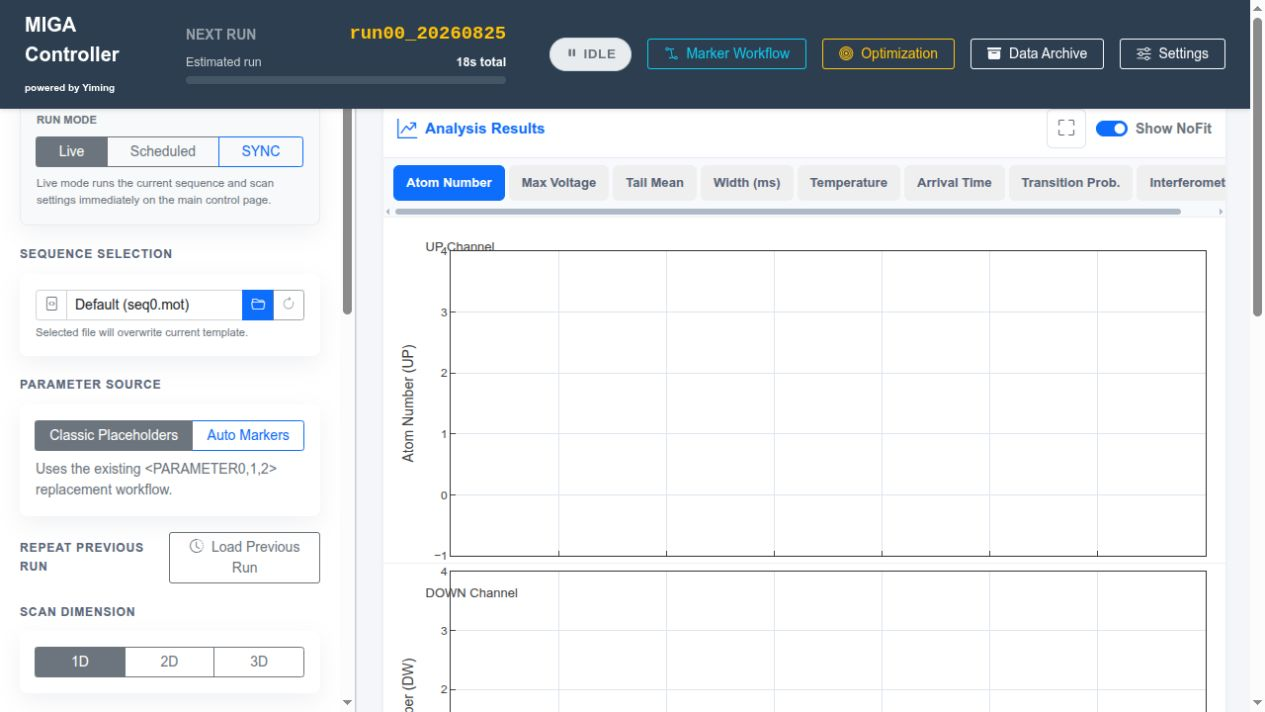
\includegraphics[width=\textwidth]{ui-control-console.jpg}
\caption{Control Console captured from the documented revision. The left pane defines
the run; the right pane shows analysis and oscilloscope output.}
\label{fig:console}
\end{figure}

\section{Run selection}
The header displays the next run ID, estimated duration and current state. \ui{Live}
starts the current configuration immediately. \ui{Scheduled} submits one or more saved
tasks to the server-side scheduler; after acceptance the browser may close. \ui{SYNC}
uses the configured master/slave topology and a shared shot plan.

\section{Sequence and parameter source}
\ui{Classic Placeholders} uses the rules in Chapter~\ref{ch:sequence}.
\ui{Auto Markers} replaces selected, validated sequence markers and can preview up to
three marker axes. The currently loaded sequence is snapshotted into every new run.
\ui{Load Previous Run} restores a saved scan configuration and, for synchronized runs,
can restore each node's sequence.

\section{Live plots}
The analysis navigation exposes Atom Number, Max Voltage, Tail Mean, Width,
Temperature, Arrival Time, Transition Probability and Interferometer. \ui{Show NoFit}
adds integration-based values where available. For multidimensional data the UI supports
surface/volume views and axis slices. The oscilloscope panels display raw and fitted UP
and DOWN traces; selecting a point associates the aggregate plot with a particular shot.

\begin{procedure}{run a bounded live scan}
  \item Confirm \ui{Live}, load the intended sequence and select the parameter source.
  \item Set the axis type, range method, start, stop, step/count and numeric type.
  \item Choose a relation mode and supply its required parameters.
  \item Set both detector fit windows; preview a waveform if the arrival time is uncertain.
  \item Set averages, randomization, external trigger and a descriptive run label.
  \item Review the estimated shot count and duration, then select \ui{START EXPERIMENT}.
  \item Watch the terminal and raw traces. Select \ui{STOP} if saturation, clipping,
  sequence errors or unexpected hardware states occur.
  \item Open the archive after completion and verify the run artifacts.
\end{procedure}

\section{Scheduled runs}
Tasks can execute sequentially with a configured gap or at scheduled timestamps. The
backend persists scheduler state. Before submission, the UI validates each task and
estimates its duration. Stopping a schedule requests termination of both the queue and
the currently active experiment.

\chapter{Signal processing and physical quantities}\label{ch:signal}

\section{Pre-processing and validation}
The acquisition driver returns a common time axis and two detector channels. Gain
correction is applied before analysis. Values exceeding the configured voltage limit are
treated as saturation/error; atom-number conversion requires at least one channel peak
to exceed the minimum signal threshold. A fit window selects the time interval used by
the nonlinear model. The raw/NoFit path uses the same stored waveform with its configured
integration rule.

\begin{figure}[htbp]
\centering
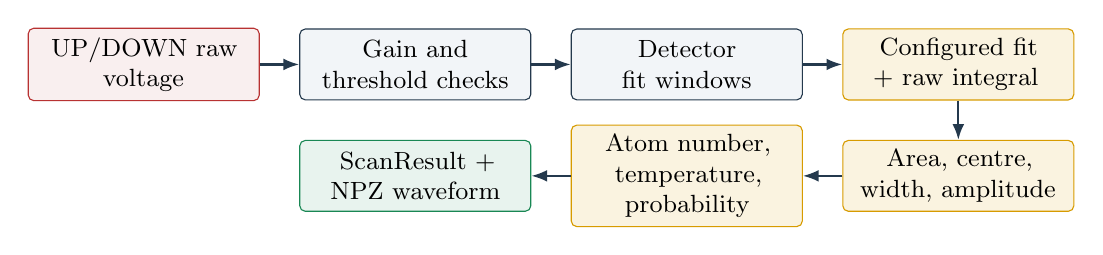
\begin{tikzpicture}[node distance=5mm]
  \node[warning] (raw) {UP/DOWN raw\\voltage};
  \node[block,right=of raw] (gain) {Gain and\\threshold checks};
  \node[block,right=of gain] (window) {Detector\\fit windows};
  \node[analysis,right=of window] (fit) {Configured fit\\+ raw integral};
  \node[analysis,below=of fit] (area) {Area, centre,\\width, amplitude};
  \node[analysis,left=of area] (physics) {Atom number,\\temperature, probability};
  \node[store,left=of physics] (result) {ScanResult +\\NPZ waveform};
  \draw[flow] (raw)--(gain); \draw[flow] (gain)--(window); \draw[flow] (window)--(fit);
  \draw[flow] (fit)--(area); \draw[flow] (area)--(physics); \draw[flow] (physics)--(result);
\end{tikzpicture}
\caption{Signal-to-physics pipeline. Fit and NoFit calculations share the calibrated
input but use different area estimators.}
\label{fig:analysis-pipeline}
\end{figure}

\section{Waveform models}
The built-in time-of-flight models include Gaussian, two skewed/modified Gaussians,
generalized Lorentzian and sinc-squared profiles. Custom models are represented by a
formula, named parameters, guess expressions, fixed/free flags and semantic roles
(amplitude, width, centre and offset). Formula syntax is parsed through a restricted AST
before numerical evaluation.

For the Gaussian model,
\begin{equation}
  V(t)=V_0+A\exp\!\left[-\frac{(t-t_0)^2}{2\sigma^2}\right],
  \qquad
  \mathcal{A}_{\mathrm{G}}=|A\sigma|\sqrt{2\pi}.
\end{equation}
Models without the Gaussian-area mode use the baseline-removed numerical integral
\begin{equation}
  \mathcal{A}_{\mathrm{fit}}=\left|\int_{t_a}^{t_b}
  \bigl[V_{\mathrm{fit}}(t)-V_0\bigr],\mathrm{d}t\right|.
\end{equation}
The edge-line NoFit method estimates a linear baseline from the first and last $n$ points
and integrates the residual. The legacy method preserves the original controller behavior.

\section{Atom-number calibration}
The conversion factor $K$ is derived in SI units from detection velocity $v_d$, wavelength
$\lambda$, light-sheet height $h_s$, transimpedance $G_T$, collection efficiency $\eta$,
photodiode responsivity $\rho$, saturation ratio $s$, detuning $\Delta$ and natural
linewidth $\Gamma$:
\begin{align}
  K &= \frac{v_d\lambda}{h_sG_T\eta h c\rho}
  \frac{2\left[1+s+(2\Delta/\Gamma)^2\right]}{\Gamma s}.
\end{align}
All positive calibration inputs are checked for finiteness and positivity.

With crosstalk coefficients $\alpha$ and $\beta$, DOWN/UP sensitivity ratio $R$ and
integrated areas $\mathcal{A}_{U,D}$,
\begin{align}
  N_{F=2} &= (\mathcal{A}_U-\alpha\mathcal{A}_D)K,\\
  N_{F=1} &= (\mathcal{A}_D-\beta\mathcal{A}_U)RK,\\
  P_{F=i} &= 100\frac{N_{F=i}}{N_{F=1}+N_{F=2}}.
\end{align}

\section{Interferometer correction}
The interferometer correction uses independent coefficients $\alpha_I$, $\beta_I$ and
$\gamma_I$. Let $n_1=N_{F=1}$ and $n_2=N_{F=2}$. Then
\begin{align}
  D &= (\beta_I-\alpha_I)(1+\gamma_I),\\
  N_1 &= \frac{\beta_I n_1-(1-\beta_I+\gamma_I)n_2}{D},\\
  N_2 &= \frac{(1-\alpha_I+\gamma_I)n_2-\alpha_I n_1}{D},\\
  P_i &= 100\frac{N_i}{N_1+N_2}.
\end{align}
If $D$ or the corrected total is numerically zero, the software returns unavailable or
zero probabilities rather than dividing by a small number.

\section{Arrival time and temperature}
For launch velocity $v_0$, target height $z$ and gravitational acceleration $g$,
\begin{equation}
  t_{\mathrm{arr}}=\frac{v_0\pm\sqrt{v_0^2-2gz}}{g}.
\end{equation}
A negative discriminant means the trajectory does not reach the target. The time-of-flight
temperature inferred from temporal width is
\begin{equation}
  T_{\mu\mathrm{K}}=10^6\frac{m_{\mathrm{Rb87}}}{k_B}
  \left(\frac{v_0}{t_{\mathrm{flight}}}-g\right)^2\sigma_t^2.
\end{equation}
The caller must supply $\sigma_t$ in the declared units; the implementation converts
milliseconds when requested.

\chapter{Sequence markers and visual editing}\label{ch:markers}

\section{Marker model}
A marker replaces a semantic quantity rather than a positional placeholder. Each
definition contains a unique ID, display name, type, decimal precision, hard minimum and
maximum, default scan start/stop/step, axis method, expected command/channel and an
optional compensation flag. Supported types are \code{dds_element}, \code{dac_value},
\code{duration} and \code{digital_state}.

Marker metadata is embedded as comments in the \code{.mot} document and is also stored in
sequence-specific profiles. The profile key prevents definitions from leaking across
unrelated sequences. The editor preserves the source encoding and line-ending convention.

\begin{figure}[htbp]
\centering
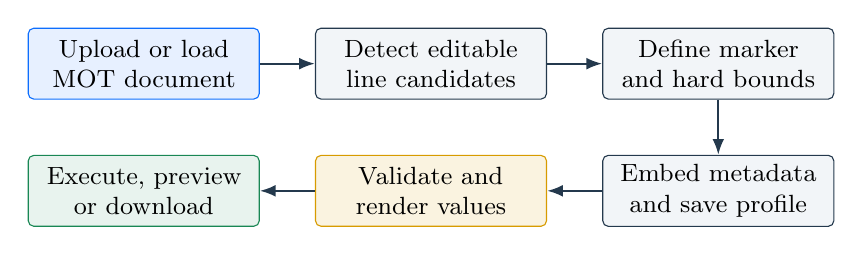
\begin{tikzpicture}[node distance=7mm]
  \node[primary] (upload) {Upload or load\\MOT document};
  \node[block,right=of upload] (inspect) {Detect editable\\line candidates};
  \node[block,right=of inspect] (define) {Define marker\\and hard bounds};
  \node[block,below=of define] (embed) {Embed metadata\\and save profile};
  \node[analysis,left=of embed] (preview) {Validate and\\render values};
  \node[store,left=of preview] (download) {Execute, preview\\or download};
  \draw[flow] (upload)--(inspect); \draw[flow] (inspect)--(define);
  \draw[flow] (define)--(embed); \draw[flow] (embed)--(preview);
  \draw[flow] (preview)--(download);
\end{tikzpicture}
\caption{Visual marker authoring and use. Marker validation is repeated at render time.}
\label{fig:marker-authoring}
\end{figure}

\section{Candidate and compensation logic}
The inspector detects editable DDS element numbers, DAC values, durations and digital
states from executable lines. Expected command and channel fields provide structural
validation. A compensation marker can update a second line when the scanned value must
preserve a total duration. Digital-state markers do not form numeric axes; each workflow
step selects Keep current, ON or OFF.

\begin{procedure}{create a marker profile}
  \item Open \ui{Settings $>$ Sequence Markers} and load the intended \code{.mot} file.
  \item Inspect candidate lines and select the exact quantity to control.
  \item Enter a descriptive name and stable uppercase ID.
  \item Choose the marker type, precision, hard bounds and safe default scan.
  \item Set expected command/channel values and a compensation line if required.
  \item Add the marker, inspect the highlighted source, and save the document profile.
  \item Download the marked file and keep it with the experimental sequence repository.
  \item Preview values at both hard limits before permitting hardware execution.
\end{procedure}

\warningtext{Renaming or moving an executable line can invalidate its embedded marker
signature. Reinspect the document after any manual sequence edit. Never widen hard limits
only to make a workflow pass validation.}

\chapter{Sequential marker optimization}\label{ch:markeropt}

\begin{figure}[htbp]
\centering
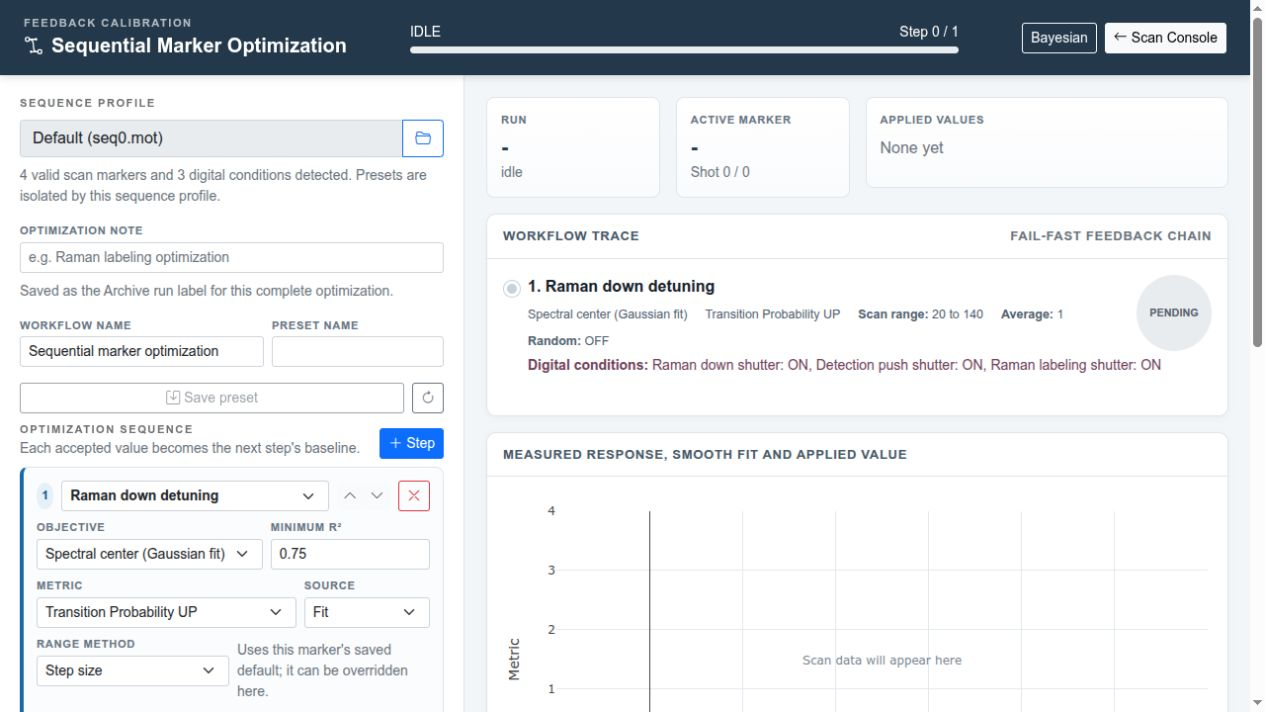
\includegraphics[width=\textwidth]{ui-marker-optimization.jpg}
\caption{Sequential Marker Optimization. Each accepted value is applied to the baseline
used by all subsequent steps.}
\label{fig:marker-ui}
\end{figure}

\section{Feedback-chain design}
Marker optimization is deterministic and ordered. A workflow step scans one numeric marker
while applying specified digital states. Repeated measurements are aggregated, the chosen
objective is evaluated, and the accepted value is written into the in-memory baseline.
If fitting or safety validation fails, execution stops before the next step.

\begin{figure}[htbp]
\centering
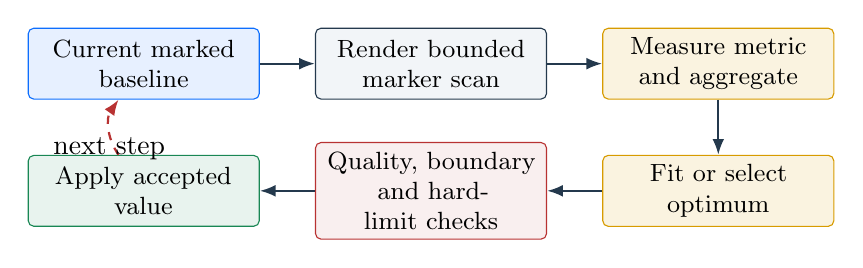
\begin{tikzpicture}[node distance=7mm]
  \node[primary] (base) {Current marked\\baseline};
  \node[block,right=of base] (scan) {Render bounded\\marker scan};
  \node[analysis,right=of scan] (measure) {Measure metric\\and aggregate};
  \node[analysis,below=of measure] (choose) {Fit or select\\optimum};
  \node[warning,left=of choose] (guard) {Quality, boundary\\and hard-limit checks};
  \node[store,left=of guard] (apply) {Apply accepted\\value};
  \draw[flow] (base)--(scan); \draw[flow] (scan)--(measure); \draw[flow] (measure)--(choose);
  \draw[flow] (choose)--(guard); \draw[flow] (guard)--(apply);
  \draw[feedback] (apply) to[bend left=35] node[below]{next step}(base);
\end{tikzpicture}
\caption{Fail-fast sequential marker optimization.}
\label{fig:marker-feedback}
\end{figure}

\section{Objectives}
Measured maximum and minimum choose an actually sampled point. Ties select the smaller
axis value. A selected endpoint is rejected because it indicates that the optimum may lie
outside the scan.

Spectral-centre fitting requires at least five distinct points and uses
\begin{equation}
  y(x)=c+A\exp\!\left[-\frac{(x-x_0)^2}{2\sigma^2}\right].
\end{equation}
The accepted value is the fitted centre $x_0$.

First-$\pi$ Rabi fitting requires at least six positive duration values and uses
\begin{equation}
  y(x)=c+A e^{-x/\tau}\sin^2\!\left(\frac{\pi x}{2t_\pi}\right).
\end{equation}
The accepted value is $t_\pi$. Both fitted objectives require
\begin{equation}
  R^2=1-\frac{\sum_i(y_i-\hat y_i)^2}{\sum_i(y_i-\bar y)^2}
  \ge R^2_{\min}.
\end{equation}
The continuous optimum must remain inside the scan. DDS elements and durations are rounded
to integers; DAC values are rounded to the marker precision. This representable value is
validated again against the scan and hard limits.

\section{Repeated measurements}
For $m$ repeats, the workflow stores every shot and reports
\begin{align}
 \bar y &= \frac{1}{m}\sum_{j=1}^m y_j,\\
 s &= \sqrt{\frac{1}{m}\sum_{j=1}^m(y_j-\bar y)^2},\\
 \mathrm{SEM} &= \frac{s}{\sqrt{m}}.
\end{align}
The implementation uses population standard deviation for repeat aggregation. The chosen
metric can come from the fitted or NoFit result.

\begin{procedure}{run a sequential marker workflow}
  \item Load a saved marker sequence profile and confirm the detected marker count.
  \item Enter a workflow name and run label; optionally load or save a preset.
  \item Add steps in physical dependency order.
  \item For each step, choose marker, objective, metric, source, scan range, average count,
  randomization and minimum $R^2$.
  \item Set every digital condition explicitly when the safe state is known.
  \item Review the complete workflow trace and confirm that every range stays within the
  stored marker hard limits.
  \item Start the workflow and inspect the measured curve, residuals and applied value.
  \item On completion, download the optimized sequence, workflow CSV and JSON report; also
  verify them in the archive.
\end{procedure}

\section{Failure behavior}
A missing metric, invalid marker, insufficient points, failed shot, poor $R^2$, out-of-range
fit, endpoint optimum or user stop prevents the current value from becoming a downstream
baseline. The archive retains completed steps and the error context for diagnosis.

\chapter{Bayesian optimization}\label{ch:bayes}

\begin{figure}[htbp]
\centering
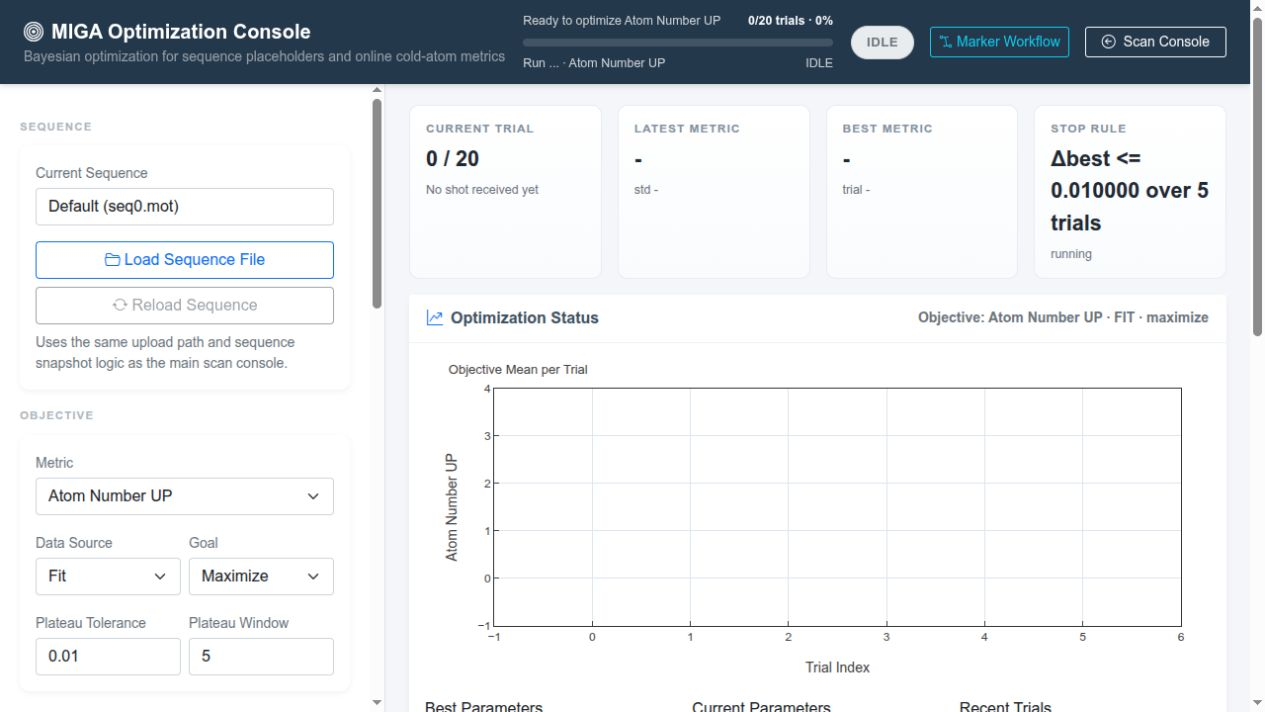
\includegraphics[width=\textwidth]{ui-bayesian-optimization.jpg}
\caption{Bayesian Optimization Console. It shows trial progress, the objective history,
the current/best parameter sets and the active stop rule.}
\label{fig:bayes-ui}
\end{figure}

\section{Search space and generation strategy}
The Bayesian workflow uses Ax. Each configured \code{PARAMETER}$n$ is an ordered discrete
choice list generated from lower bound, upper bound and step. Integer variables are rounded;
floating variables are rounded to six decimals. A single variable is limited to 5000 grid
values. The optional initial guess is snapped to the closest legal grid point.

The Ax client configures an experiment, an initialization budget and the scalar objective
\code{optimization_score}. If no initial guess exists and the requested random budget is
zero, at least one initialization trial is retained. Measured value is also reported as a
tracking metric where the installed Ax API supports it.

\begin{figure}[htbp]
\centering
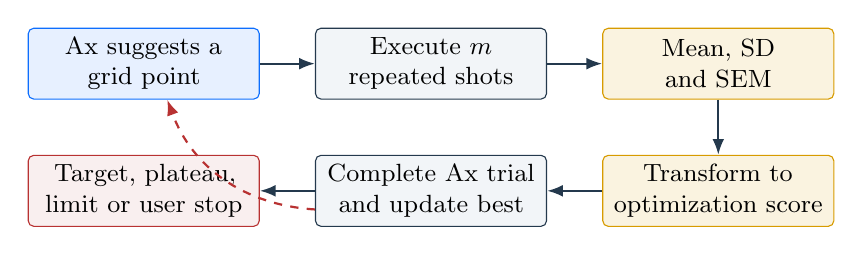
\begin{tikzpicture}[node distance=7mm]
  \node[primary] (ax) {Ax suggests a\\grid point};
  \node[block,right=of ax] (shots) {Execute $m$\\repeated shots};
  \node[analysis,right=of shots] (stats) {Mean, SD\\and SEM};
  \node[analysis,below=of stats] (score) {Transform to\\optimization score};
  \node[block,left=of score] (complete) {Complete Ax trial\\and update best};
  \node[warning,left=of complete] (stop) {Target, plateau,\\limit or user stop};
  \draw[flow] (ax)--(shots); \draw[flow] (shots)--(stats); \draw[flow] (stats)--(score);
  \draw[flow] (score)--(complete); \draw[flow] (complete)--(stop);
  \draw[feedback] (complete) to[bend left=33] (ax);
\end{tikzpicture}
\caption{Bayesian optimization loop. Hardware evaluation remains the dominant operation;
Ax only selects the next legal parameter tuple.}
\label{fig:bayes-loop}
\end{figure}

\section{Objective scoring}
Let $\bar y$ be the repeat mean. The internal score maximized by Ax is
\begin{equation}
  q(\bar y)=
  \begin{cases}
    \bar y, & \text{maximize},\\
    -\bar y, & \text{minimize},\\
    -|\bar y-y_\star|, & \text{target}.
  \end{cases}
\end{equation}
Supported metrics include UP/DOWN atom number, amplitude, temperature, arrival time,
transition probability and interferometer populations/probabilities. The source can be Fit
or NoFit.

Target mode stops when $|\bar y-y_\star|$ is no greater than the target tolerance. Maximize
and minimize modes can stop on a plateau. If $q_k^\mathrm{best}$ is the best score after
trial $k$, a window $w$ stops when
\begin{equation}
  q_k^\mathrm{best}-q_{k-w}^\mathrm{best}\le\epsilon_{\mathrm{plateau}}.
\end{equation}

\begin{procedure}{run Bayesian optimization}
  \item Perform a manual bounded scan for each candidate variable.
  \item Load the same sequence into the Optimization Console.
  \item Select metric, Fit/NoFit source and maximize/minimize/target goal.
  \item Add unique \code{PARAMETER} indices with legal bounds, grid step and type.
  \item Choose repeat count, maximum trials and initial random trials.
  \item Configure either target tolerance or plateau tolerance/window.
  \item Start the run and monitor objective dispersion as well as the mean.
  \item Export \pathcode{optimization_history.csv}, \pathcode{optimization_report.json}
  and the best rendered sequence.
\end{procedure}

\notetext{A low mean uncertainty does not prove that the global optimum was found. Search
quality depends on the bounded grid, metric stability, initialization and trial budget.}

\chapter{Bragg, AC Stark, lock-in and transfer-function workflows}\label{ch:special}

\section{Calibrated Bragg pulse generation}
The Bragg generator writes channel 32 with a sampled Gaussian or Blackman envelope. For a
Gaussian FWHM $w$,
\begin{equation}
  \sigma=\frac{w}{2\sqrt{2\ln2}},\qquad t\in[0,8\sigma].
\end{equation}
For a Blackman envelope, total duration is $w/0.405$. Samples use the configured clock
resolution (default \SI{0.2}{\micro\second}). Two off samples are included, so the timing
compensation is
\begin{equation}
  P_1=t_{\mathrm{base}}-(N_{\mathrm{sample}}+2)\Delta t.
\end{equation}
Negative compensation and more than two million samples are rejected.

Normalized optical power is converted to voltage by inverting a generalized logistic
calibration. For voltage $v$,
\begin{equation}
  P(v)=L+(U-L)\left[1+e^{-k(v-v_0)}\right]^{-\nu}.
\end{equation}
The selected linear voltage interval is renormalized to $[0,1]$. Requests below the off
threshold map to \SI{-3}{V}; operating voltages must remain within \SIrange{-15}{15}{V}.

\section{AC Stark centering}
The AC Stark workflow validates an uploaded \code{ad9958} XML table and appends one DDS
element per requested Raman power ratio $r=P_{R1}/P_{R2}$. At constant total power,
\begin{equation}
 P_{R1}=P_{\mathrm{tot}}\frac{r}{1+r},\qquad
 P_{R2}=P_{\mathrm{tot}}\frac{1}{1+r}.
\end{equation}
Each power is inverted through its own generalized-logistic amplitude calibration and
rounded to an integer in $[0,1023]$. The actual powers and ratio are recalculated from the
rounded amplitudes and archived. XML element numbers and counts are limited to 500.

The workflow interleaves left and right sequence points, writes and verifies the generated
DDS table, performs the measurements, then attempts to restore the original table. Both
the original and generated XML plus the ratio plan are stored with the run.

\warningtext{If DDS restoration reports an error, stop dependent experiments and verify
the physical DDS state with the site procedure before running another sequence.}

\section{ABBA digital lock-in}
Lock-in mode creates complete four-shot blocks with states A--B--B--A. The reference vector is
\begin{equation}
 \mathbf{r}=(+1,-1,-1,+1).
\end{equation}
For signals $S_1,\ldots,S_4$,
\begin{align}
 S_A&=\frac{S_1+S_4}{2}, &
 S_B&=\frac{S_2+S_3}{2},\\
 X&=\frac{S_1-S_2-S_3+S_4}{4},\\
 R&=\frac{S_A-S_B}{S_A+S_B},\\
 E&=S_A-2S_B, &
 E_N&=\frac{S_A-2S_B}{S_A+2S_B}.
\end{align}
Only complete blocks with the expected states and references contribute. Each supported
Fit and NoFit metric receives block values plus mean, sample standard deviation and SEM.

\begin{figure}[htbp]
\centering
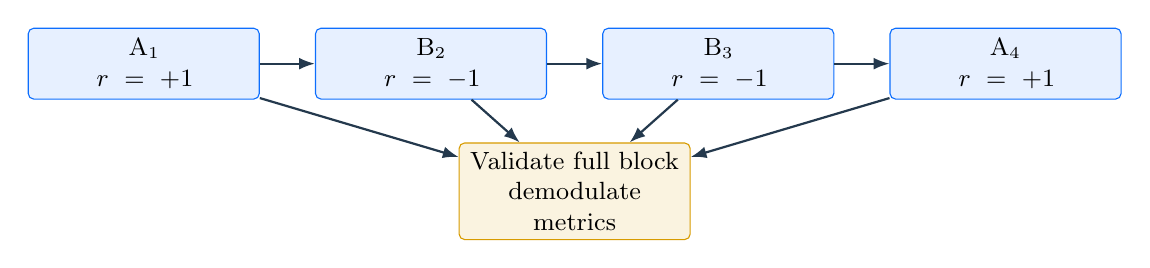
\begin{tikzpicture}[node distance=7mm]
  \node[primary] (s1) {A$_1$\\$r=+1$};
  \node[primary,right=of s1] (s2) {B$_2$\\$r=-1$};
  \node[primary,right=of s2] (s3) {B$_3$\\$r=-1$};
  \node[primary,right=of s3] (s4) {A$_4$\\$r=+1$};
  \node[analysis,below=10mm of $(s2)!0.5!(s3)$] (demod) {Validate full block\\demodulate metrics};
  \draw[flow] (s1)--(s2); \draw[flow] (s2)--(s3); \draw[flow] (s3)--(s4);
  \draw[flow] (s1)--(demod); \draw[flow] (s2)--(demod);
  \draw[flow] (s3)--(demod); \draw[flow] (s4)--(demod);
\end{tikzpicture}
\caption{ABBA lock-in block and reference sequence.}
\label{fig:abba}
\end{figure}

\section{Bragg transfer-function scan}
Transfer Function is a Live, one-dimensional, ordered scan of the carrier frequency on
a selected channel of an Aim-TTi TG5012A or TGF3162. Configure the model, channel and
instrument address under \ui{Settings $>$ TTI Generator}, select Transfer Function under \ui{Scan Logic}, and enter the
frequency start, stop, step and repetitions per frequency. The uploaded \code{.mot}
sequence is executed unchanged and therefore requires no \code{PARAMETER} placeholder.
The TTI Generator settings tab also provides a test-frequency action: it connects with the
currently displayed address, verifies the selected model and immediately sets only the selected channel's
carrier frequency. The previous frequency is not restored.

The controller opens one instrument LAN connection on TCP port 9221 for the scan. At each
new frequency it selects the configured channel and sends only the \code{FREQ} command.
TG5012A waits for the instrument's operation-complete reply; TGF3162 uses the established
fire-and-forget write because some firmware does not reliably answer \code{*OPC?}. The
controller then waits a fixed five seconds before the first sequence. It does not
change waveform, amplitude, phase or output state and does not restore the original
frequency after the scan.

For every frequency, the live and Archive plots show the sample standard deviation
($n-1$ denominator) of atom number, interferometer probabilities $P_1/P_2$, and calibrated
interferometer phase. Fit is the default source; NoFit is available for atom number and
$P_1/P_2$. Phase follows the active calibration snapshot for the run. One complete
frequency sweep is stored as one Archive run, including every shot and waveform plus
\pathcode{transfer_function_summary.csv} and
\pathcode{transfer_function_summary.json}.

\chapter{Synchronized multi-controller operation}\label{ch:sync}

\section{Roles and authorization}
A controller is configured as Standalone, Master or Slave. The master stores a list of
enabled slaves with node IDs, names, base URLs and per-node sequences. Requests can carry
a shared token; a slave may also restrict the allowed master IP. The \ui{Test} action
checks reachability before a run.

\section{Prepare, start and pair}
The master generates the complete scan once and serializes it as a shot plan. Each slave
receives the run ID, master/slave IDs, scan configuration, shot plan and sequence content
(text or base64 for binary-safe transfer). Every slave must report ready before any start
command is sent. Slaves start first; the master begins after the configured delay.

\begin{figure}[htbp]
\centering
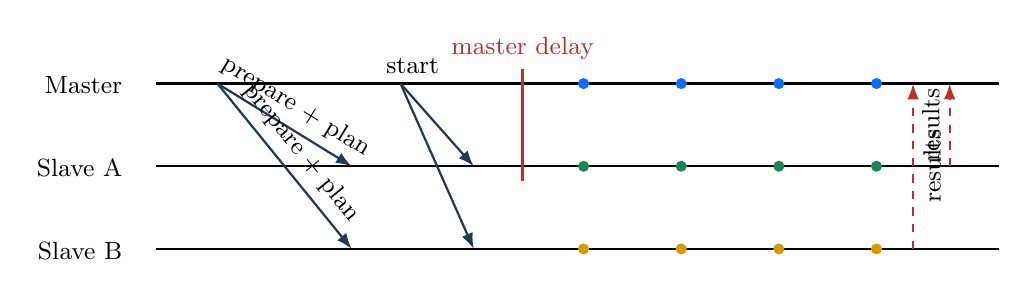
\begin{tikzpicture}[x=1.55cm,y=0.75cm,font=\small]
  \node[anchor=e] at (0,0) {Master};
  \node[anchor=e] at (0,-1.4) {Slave A};
  \node[anchor=e] at (0,-2.8) {Slave B};
  \draw[thick] (0.2,0)--(7.1,0);
  \draw[thick] (0.2,-1.4)--(7.1,-1.4);
  \draw[thick] (0.2,-2.8)--(7.1,-2.8);
  \draw[flow] (0.7,0)--node[above,sloped]{prepare + plan}(1.8,-1.4);
  \draw[flow] (0.7,0)--node[above,sloped]{prepare + plan}(1.8,-2.8);
  \draw[flow] (2.2,0)--(2.8,-1.4); \draw[flow] (2.2,0)--(2.8,-2.8);
  \node[above] at (2.3,0) {start};
  \draw[MigaRed,very thick] (3.2,-1.65)--(3.2,0.25);
  \node[above,text=MigaRed] at (3.2,0.25) {master delay};
  \foreach \x in {3.7,4.5,5.3,6.1}{
    \fill[MigaBlue] (\x,0) circle (2pt);
    \fill[MigaGreen] (\x,-1.4) circle (2pt);
    \fill[MigaGold] (\x,-2.8) circle (2pt);
  }
  \draw[feedback] (6.7,-1.4)--node[above,sloped]{results}(6.7,0);
  \draw[feedback] (6.4,-2.8)--node[below,sloped]{results}(6.4,0);
\end{tikzpicture}
\caption{Master/slave synchronization. Pairing uses logical shot index, not network
arrival order.}
\label{fig:sync-timeline}
\end{figure}

Master and slave results are keyed by \code{sync_shot_index}. A pair is emitted only when
both sides exist and neither contains an error. The UI can display per-node curves or
differential paired results and replay completed points.

\section{Archive replication}
Each node first writes a normal local archive. A ZIP bundle excludes temporary files and
nested sync copies. SHA-256 checksums protect transfer integrity. Extraction rejects path
traversal, stages files in a temporary directory, requires both \pathcode{results.csv} and
\pathcode{config.json}, and atomically replaces the previous node copy. The final master
archive contains \pathcode{sync_nodes/<node-id>/} and a sync manifest. Replication is
bidirectional; failed transfers can be retried from the archive interface.

\begin{procedure}{run a synchronized scan}
  \item Configure one Master and one or more Slaves with the same shared token.
  \item Test every enabled slave from \ui{Settings $>$ SYNC}.
  \item In the Control Console select \ui{SYNC}, load the master sequence and each slave
  sequence, then configure a bounded scan.
  \item Set master delay according to the physical trigger arrangement.
  \item Start and confirm that all nodes enter ready/running states.
  \item Monitor paired count, per-node progress and differential plots.
  \item After completion, open the master archive, select every node and verify archive
  replication status. Retry incomplete transfers.
\end{procedure}

\chapter{Data archive and re-analysis}\label{ch:archive}

\begin{figure}[htbp]
\centering
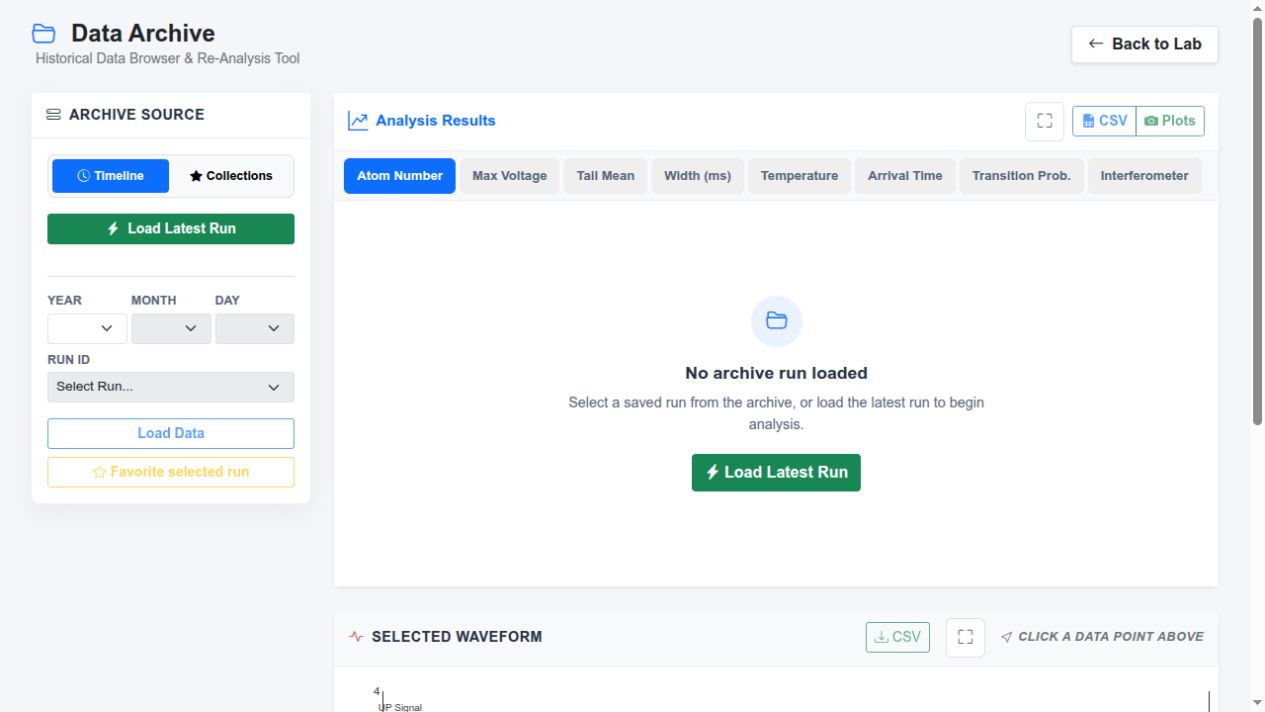
\includegraphics[width=\textwidth]{ui-data-archive.jpg}
\caption{Data Archive before a run is loaded. Timeline and Collections provide two paths
to the same immutable run data.}
\label{fig:archive-ui}
\end{figure}

\section{Archive structure}
Runs are organized by year, month and day. A typical directory is
\begin{lstlisting}
Data_log/2026/08/25/run00_20260825/
  config.json
  results.csv
  sequence.mot
  waveforms/step_0001.npz
  sync_manifest.json              # synchronized runs only
  sync_nodes/<node-id>/...         # replicated node archives
\end{lstlisting}
The configuration is a reproducibility snapshot. \pathcode{results.csv} provides fast
aggregate loading. Each NPZ stores time, raw UP/DOWN, fitted UP/DOWN and fit-window arrays.

\section{Timeline and collections}
Timeline browsing selects year, month, day and run. Collections are SQLite-backed folders
containing favourites. A favourite can have an alias, note, preview metric and preview
step. Batch operations support moving or removing selected favourites without changing the
underlying experiment directory.

\section{Re-analysis}
Recalculation loads the raw waveform, normalizes new analysis settings, reapplies gain and
fit windows, runs the selected fit model and recomputes physics metrics. The display can
switch between saved and recalculated results. \ui{Overwrite} updates calculated archive
products only when the user explicitly requests it; raw NPZ waveforms remain the primary
evidence.

\section{Scan fitting}
Aggregate curves can be fitted over a selected $x$ range. Built-in scan models are Gaussian,
Lorentzian, Rabi oscillation, atom-interferometer fringes, Bragg fringes and Custom. The
model editor defines formula, parameter guesses, fixed flags and semantic roles. Fit curves
are evaluated on 32--4000 points for display. A custom model should first be tested on a
copy of a run.

\begin{figure}[htbp]
\centering
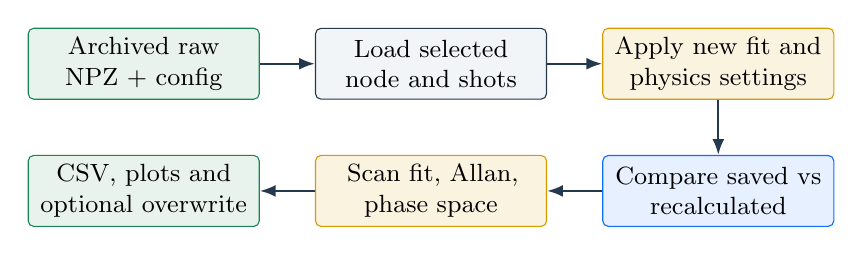
\begin{tikzpicture}[node distance=7mm]
  \node[store] (disk) {Archived raw\\NPZ + config};
  \node[block,right=of disk] (load) {Load selected\\node and shots};
  \node[analysis,right=of load] (recalc) {Apply new fit and\\physics settings};
  \node[primary,below=of recalc] (view) {Compare saved vs\\recalculated};
  \node[analysis,left=of view] (scanfit) {Scan fit, Allan,\\phase space};
  \node[store,left=of scanfit] (export) {CSV, plots and\\optional overwrite};
  \draw[flow] (disk)--(load); \draw[flow] (load)--(recalc); \draw[flow] (recalc)--(view);
  \draw[flow] (view)--(scanfit); \draw[flow] (scanfit)--(export);
\end{tikzpicture}
\caption{Archive re-analysis preserves raw evidence while allowing new derived products.}
\label{fig:archive-flow}
\end{figure}

\chapter{Bragg fringe, phase space and stability}\label{ch:stability}

\section{Bragg fringe acceleration fit}
With $x=T^2$ expressed in \si{\micro\second\squared}, the model is
\begin{equation}
  y(x)=C+A\cos(\omega x+\phi_0),\qquad
  k_{\mathrm{eff}}=\frac{4\pi n}{\lambda}.
\end{equation}
For a fixed candidate $\omega$, the offset and cosine/sine coefficients form a linear
least-squares problem. The implementation scans a bounded frequency grid, refines the best
candidates with scalar minimization, and rejects frequencies above the sampling limit or
the acceleration projection of standard gravity. It then reports
\begin{equation}
  a=\frac{\omega\,10^{12}}{k_{\mathrm{eff}}},\qquad
  \theta=10^3\arcsin\!\left(\frac{a}{g_0}\right)\ \mathrm{mrad}.
\end{equation}
Mid-fringe locations satisfy
\begin{equation}
  x_j=\frac{\pi/2+j\pi-\phi_0}{\omega},\qquad
  \Delta x_{\mathrm{mid}}=\frac{\pi}{\omega}.
\end{equation}
Valid Bragg fit results can be saved as named reusable phase calibrations.

\section{Phase-space conversion}
For a measured value $y_i$, calibration amplitude $A$ and corrected offset $C$, the
normalized signal is clipped for inversion:
\begin{equation}
  z_i=\operatorname{clip}\!\left(\frac{y_i-C}{A},-1,1\right).
\end{equation}
Because $\arccos z$ is multi-valued, the software enumerates both signs and neighboring
$2\pi$ cycles, then chooses the phase nearest the prediction
$\phi_i^{\mathrm{pred}}=\omega P_{0,i}+\phi_0$ or a fixed mid-fringe reference. The wrapped
deviation is $\delta\phi_i=\operatorname{wrap}(\phi_i-\phi_i^{\mathrm{pred}})$.

Sensitivity is $|\sin\phi_i^{\mathrm{pred}}|$. A point is high quality only when it is
inside the user-defined mid-fringe band and its normalized signal was not clipped. Optional
reference-first correction shifts $C$ by the mean residual of the first $N$ points.

\section{Archive interferometer phase and SYNC $A/C$ optimization}
\subsection{Monotonic half-fringe phase conversion}
The Archive interferometer-phase view uses each node's own effective Bragg calibration.
For a SYNC archive this is normally the calibration snapshot saved by that node; an
archive phase-reference override, when present, becomes the effective calibration. The
selected signal field (for example \code{intf_p1} or \code{intf_p1_nofit}), slope,
$\omega$, $\phi_0$ and reference $T^2$ therefore remain independent for Master and Slave.

For measured signal $S_{i,k}$ from node $i$ and shot $k$, define
\begin{equation}
  u_{i,k}=\frac{S_{i,k}-C_i}{A_i}.
\end{equation}
Unlike the general phase-space display above, Archive interferometer phase does not clip
an out-of-envelope value: $|u_{i,k}|>1$ makes the shot invalid. A saved monotonic-slope
choice selects one $\pi$-wide half-fringe. With
\begin{equation}
  s_i=\begin{cases}
    +1,&\text{negative-slope half-fringe},\\
    -1,&\text{positive-slope half-fringe},
  \end{cases}
\end{equation}
the reported phase relative to the calibration reference is
\begin{equation}
  \Delta\phi_{i,k}
  =s_i\arccos(u_{i,k})
  -s_i\arccos\!\left[\cos\!\left(\omega_iT_{i,\mathrm{ref}}^2+\phi_{0,i}\right)\right].
  \label{eq:archive-phase}
\end{equation}
SYNC rows are paired by logical shot index and matching $P_0=T^2$. For selected Reference
and Target nodes the differential sequence is
\begin{equation}
  d_k=\Delta\phi_{\mathrm{Target},k}-\Delta\phi_{\mathrm{Reference},k}.
\end{equation}
The ordinary series view wraps the difference to $(-\pi,\pi]$. Optimization unwraps the
chronological sequence because the expected physical differential phase is an unknown
constant and a wrap boundary must not create artificial noise.

\subsection{Why optimize $A$ and $C$}
Equation~\eqref{eq:archive-phase} shows that changing only $\omega$ or $\phi_0$ changes a
constant reference term and therefore cannot change standard deviation or first-order
Allan deviation. Amplitude and offset change the per-shot nonlinear inversion. Their
local sensitivities are
\begin{equation}
  \frac{\partial\Delta\phi}{\partial A}
  =s\frac{u}{A\sqrt{1-u^2}},\qquad
  \frac{\partial\Delta\phi}{\partial C}
  =s\frac{1}{A\sqrt{1-u^2}}.
\end{equation}
At mid-fringe $u\simeq0$, $C$ is directly constrained while the first-order sensitivity
to $A$ is weak. The saved fringe curve and parameter prior are consequently essential
when estimating $A$ from a mid-fringe-only SYNC sequence.

The optimizer varies four independent parameters,
\begin{equation}
  \mathbf p=(A_R,C_R,A_T,C_T),
\end{equation}
starting from the Reference and Target nodes' respective effective calibrations. It keeps
$\omega$, $\phi_0$, reference $T^2$, monotonic slope and signal-source selection fixed.
Reversing the displayed difference swaps Reference and Target roles but never causes the
nodes to share calibration parameters.
The Archive page submits the selected nodes and controls to
\code{/archive/sync-phase-calibration-optimize}; the server reads the paired raw signal
fields and both effective calibrations from the selected archive.

\subsection{Objective and constraints}
The selectable SYNC metric $m(d)$ is
\begin{equation}
  m(d)=\begin{cases}
    \sigma_{\mathrm{A},1}(d),&\text{Allan n=1},\\
    \operatorname{std}(d),&\text{Standard deviation},\\
    \sqrt{\lambda\sigma_{\mathrm{A},1}^2(d)+(1-\lambda)\operatorname{std}^2(d)},
      &\text{Combined},
  \end{cases}
\end{equation}
where $\lambda$ is \ui{Allan Weight}. The first-order value is
\begin{equation}
  \sigma_{\mathrm{A},1}(d)
  =\sqrt{\frac{1}{2(N-1)}\sum_{k=1}^{N-1}(d_{k+1}-d_k)^2}.
\end{equation}
The normalized optimization loss is
\begin{equation}
  L=\left(\frac{m(d)}{m(d_0)}\right)^2
  +w_fL_{\mathrm{fringe}}+w_pL_{\mathrm{prior}}+L_{\mathrm{invalid}},
  \label{eq:sync-ac-loss}
\end{equation}
where $d_0$ is the sequence produced by the original calibrations. For node $i$, candidate
$A_i,C_i$ are compared with that node's own saved fitted curve $(x_j,y_j^{\mathrm{fit}})$:
\begin{align}
  \widehat y_{i,j}&=C_i+A_i\cos(\omega_ix_j+\phi_{0,i}),\\
  L_{\mathrm{fringe}}&=
  \left(\frac{\operatorname{RMSE}_R}{A_{R,0}}\right)^2+
  \left(\frac{\operatorname{RMSE}_T}{A_{T,0}}\right)^2.
\end{align}
Thus \ui{Fringe Weight} $w_f$ controls how strongly the optimized curves must remain close
to the two saved fitting curves. The current constraint uses saved \code{fit_x}/
\code{fit_y}; it does not refit the original raw fringe shots.

For an \ui{A/C Bounds} fraction $b$, the hard parameter intervals are
\begin{align}
  A_i&\in[A_{i,0}(1-b),A_{i,0}(1+b)],\\
  C_i&\in[C_{i,0}-bA_{i,0},C_{i,0}+bA_{i,0}].
\end{align}
The soft prior is the mean squared displacement normalized by these allowed scales,
\begin{equation}
  L_{\mathrm{prior}}=\frac{1}{4}\sum_q
  \left(\frac{p_q-p_{q,0}}{bA_{i(q),0}}\right)^2.
\end{equation}
\ui{Prior Weight} $w_p$ therefore controls direct preference for the original $A,C$
values, whereas \ui{Fringe Weight} controls agreement with the original curves. Candidate
parameters that make a normalized signal leave $[-1,1]$ receive an overflow and invalid-
shot penalty; invalid shots are not silently removed to improve the objective.

Recommended initial controls are $b=10\%$, $w_f=1$ and $w_p=0.05$. Reducing the weights
allows more aggressive SYNC-noise reduction; increasing them makes the result more
conservative. Do not set both weights to zero for mid-fringe data. A parameter reaching
its hard boundary is reported and normally indicates that the bound, data model or
calibration quality needs review rather than automatic acceptance.

\begin{procedure}{preview a joint SYNC $A/C$ optimization}
  \item Load a replicated SYNC run in the Data Archive and select
  \ui{Interferometer Phase}.
  \item Select exactly two hosts. The first is Reference and the second Target; use
  \ui{Reverse Difference} when required.
  \item Set the inclusive $P_0$ range to the chronological shots that should constrain
  the constant differential phase.
  \item In \ui{Joint A/C calibration optimization}, choose \ui{Allan n=1},
  \ui{Standard deviation} or \ui{Combined}; then set bounds and constraint weights.
  \item Click \ui{Optimize A/C}. Inspect parameter changes, valid-pair count, boundary
  warnings, saved-curve RMSE and the mean-removed before/after differential plot.
  \item The optimized per-node phases immediately feed the existing Phase Series, Allan
  plot and Sequence Statistics. Changing Allan order or $P_0$ filtering recalculates
  those views from the preview values.
  \item Click \ui{Reset preview} to restore the archived phases.
\end{procedure}

\warningtext{Optimization results are preview-only. They do not overwrite an archived
run and do not save or activate a Settings calibration. A small Allan or standard
deviation alone is insufficient evidence of a valid calibration: also inspect curve
agreement, parameter movement, valid-shot count and boundary warnings.}

\section{Overlapping Allan deviation}
Allan analysis is available only for non-randomized one-dimensional scans. After optional
inclusive $P_0$ filtering, for averaging order $n$ define adjacent block means
\begin{equation}
  \bar y_i^{(n)}=\frac{1}{n}\sum_{j=0}^{n-1}y_{i+j}.
\end{equation}
The overlapping Allan deviation is
\begin{equation}
  \sigma_y(n)=\sqrt{\frac{1}{2M}\sum_{i=1}^{M}
  \left(\bar y_{i+n}^{(n)}-\bar y_i^{(n)}\right)^2},
\end{equation}
where only windows whose $2n$ samples are finite contribute. The maximum order is half the
filtered sequence length. The UI supports absolute or mean-normalized values, linear or
logarithmic order axes, and displays valid-window count, mean, RMS and sample standard
deviation for Fit and raw channels.

\chapter{Settings, calibration and maintenance}\label{ch:settings}

\begin{figure}[htbp]
\centering
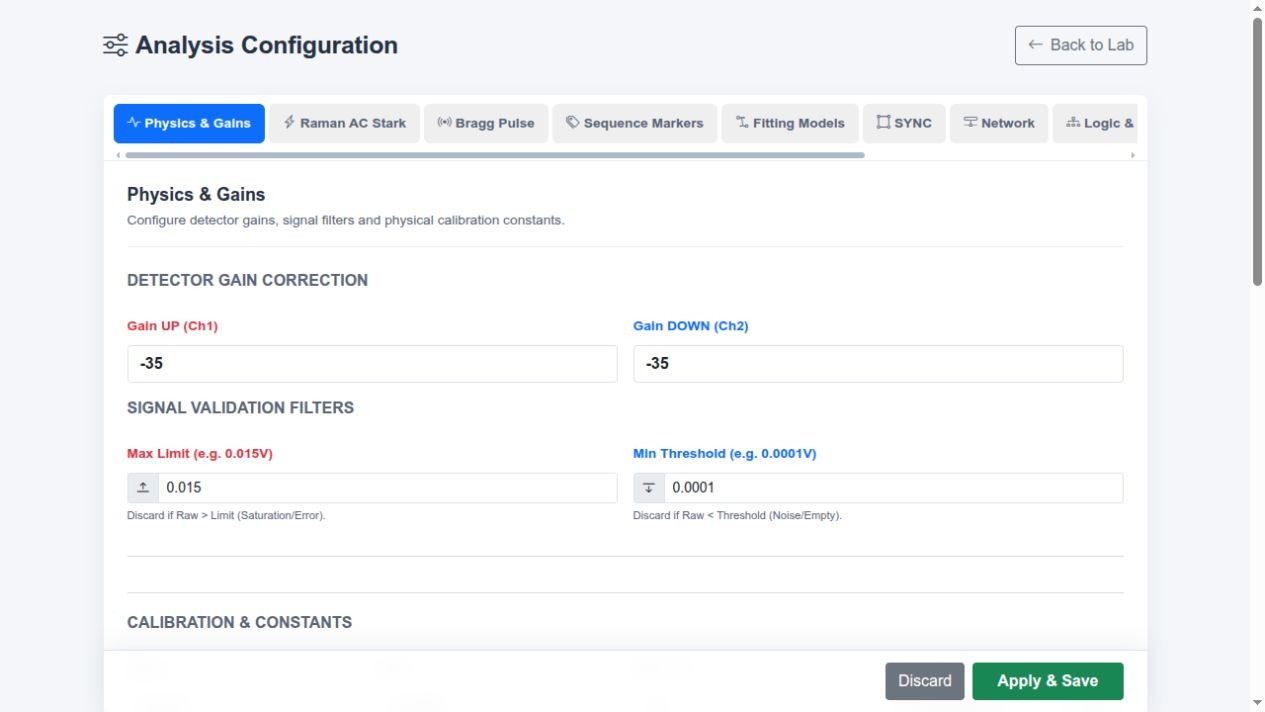
\includegraphics[width=\textwidth]{ui-settings.jpg}
\caption{Settings interface. Tabs separate physical calibration from execution, network
and maintenance concerns.}
\label{fig:settings-ui}
\end{figure}

\begin{longtable}{>{\bfseries}p{0.20\textwidth} p{0.72\textwidth}}
\caption{Settings tabs and responsibilities.}\label{tab:settings}\\
\toprule
Tab & Responsibility\\
\midrule
\endfirsthead
\toprule Tab & Responsibility\\ \midrule
\endhead
Physics \& Gains & Detector gains, validation limits, $K$ inputs, crosstalk, geometry,
launch velocity, decimation and interferometer coefficients.\\
Raman AC Stark & DDS writer path and four independent R1/R2 amplitude-to-power
calibrations for UP and DOWN groups.\\
Bragg Pulse & Channel-32 voltage-to-power logistic calibration, linear interval and off
threshold, with raw and normalized preview plots.\\
Sequence Markers & Visual marker editor, saved documents, definitions, hard bounds,
compensation and embedded metadata.\\
Fitting Models & Atom-area method, baseline points, waveform model formulas, guesses,
roles and fixed/free parameters.\\
SYNC & Standalone/Master/Slave role, node name, token, allowed IP and slave endpoints.\\
TTI Generator & TG5012A/TGF3162 selection, CH1/CH2 selection, direct instrument IP, TCP
port, timeout, connection test and frequency test for Transfer Function scans.\\
Network & Acquisition platform, Red Pitaya addresses, DAQ rate and timeout.\\
Logic \& Channels & Launch/trigger channel IDs and linked-mode timing constant.\\
System Paths & \code{tmot4}, arguments, \code{cmot4}, default template and DDS writer.\\
System Update & Repository URL, branch, fetch status and controlled update action.\\
\bottomrule
\end{longtable}

Settings are saved to \pathcode{user_settings.json}. The manager refreshes runtime settings
from disk before starting optimization. Keep a versioned laboratory copy of calibration
values, but do not commit host-specific credentials or tokens.

\begin{procedure}{calibration change control}
  \item Export or copy the existing settings and record the current run reference.
  \item Change one calibration family at a time.
  \item Use preview plots and a known reference sequence to validate the direction and
  range of the response.
  \item Record the calibration source, date, apparatus state and valid interval.
  \item Run a small validation scan and retain its archive before using the calibration in
  optimization or scheduled operation.
\end{procedure}

\chapter{Data products and exports}\label{ch:data}

\begin{table}[htbp]
\centering
\caption{Principal reproducibility artifacts.}
\begin{tabularx}{\textwidth}{l X}
\toprule
Artifact & Contents\\
\midrule
\pathcode{config.json} & Complete run configuration and analysis/settings snapshot.\\
\pathcode{results.csv} & Per-shot parameters, Fit/NoFit metrics, mode metadata and errors.\\
\pathcode{sequence.mot} & Exact sequence snapshot used by the run.\\
\pathcode{waveforms/step_NNNN.npz} & Time axis, raw and fitted channels, fit windows.\\
Marker workflow CSV/JSON & Step definitions, repeated values, fits, selected/applied values
and error state.\\
Optimized marker sequence & Final baseline after all accepted marker steps.\\
\pathcode{optimization_history.csv} & Trial parameters, mean, SD, SEM, score and best-so-far.\\
\pathcode{optimization_report.json} & Optimization configuration and final status.\\
Best sequence & Classic placeholder template rendered with best Bayesian parameters.\\
AC Stark XML and plan & Original/generated DDS tables and requested/actual power ratios.\\
Transfer Function CSV/JSON & Per-frequency valid sample counts, means and sample standard
deviations for Fit, NoFit and calibrated phase metrics.\\
\pathcode{sync_manifest.json} & Node identities, progress, paired data and replication state.\\
\bottomrule
\end{tabularx}
\end{table}

To reproduce a numerical result, retain the raw waveform, configuration snapshot, exact
sequence, software revision and any external hardware calibration or firmware version that
is not stored by the controller. A plot image or CSV alone is insufficient.

\chapter{Troubleshooting}\label{ch:trouble}

\small
\begin{longtable}{p{0.23\textwidth} p{0.29\textwidth} p{0.40\textwidth}}
\caption{Symptom-oriented troubleshooting guide.}\label{tab:trouble}\\
\toprule
Symptom & Likely cause / check & Corrective action\\
\midrule
\endfirsthead
\toprule Symptom & Likely cause / check & Corrective action\\ \midrule
\endhead
Controller does not start & Wrong interpreter, missing package, stale launcher state or
occupied port. & Run \code{--check-only} and \code{--status}; inspect
\pathcode{.launcher_state/server.log}; stop the known prior process before changing ports.\\
Ax import failure & Backend started outside \pathcode{.venv} or \code{ax-platform} is
missing. & Start through \code{launch_code} or \code{start_controller.sh}; repair the
virtual environment rather than installing Ax only for root/system Python.\\
Compiler path error & \code{tmot4}, \code{cmot4} or template path is missing/not
executable. & Use \ui{System Paths} auto-fill, then verify each resolved file and execute
permission.\\
Compilation fails & Invalid MOT syntax, unresolved placeholder, or unsupported marker
rendering. & Download/preview the rendered sequence, run the compiler manually, and inspect
the first reported source line.\\
VCD timing unavailable & Launch/trigger channel IDs do not exist in compiled VCD. & Match
\ui{Logic \& Channels} to the actual sequence channel numbers and recompile.\\
DAQ timeout & Wrong IP/platform, network route, too-short timeout or device busy. & Test the
device independently, confirm the selected platform, increase timeout within laboratory
policy and retry a single simulation shot first.\\
Waveform rejected & Peak exceeds voltage limit or both channels remain below minimum. &
Inspect raw traces; correct optical/electronic gain and thresholds. Do not simply widen
limits around a saturated detector.\\
Fit fails & Empty/incorrect fit window, too few samples, poor initial guess or unsuitable
model. & Display raw data, move the window, select a physically suitable model and test
with fixed/simple parameters.\\
NoFit disagrees strongly & Baseline drift or inappropriate area method. & Compare legacy
and edge-line integration, increase baseline points cautiously, and inspect the waveform
edges.\\
Link formula error & Invalid expression/name or dependency order. & Use only $P_0$, earlier
$P_i$, \code{math} and \code{np}; evaluate formulas one at a time.\\
Marker not detected & Target line is not executable, signature changed or profile differs.
& Reopen the original MOT in the visual editor, inspect candidates and save a new profile.\\
Embedded metadata invalid & Manual comment corruption or conflicting definitions. & Keep a
copy, remove/recreate the affected marker through the editor, then download the repaired
document.\\
Compensation rejected & Second line missing, wrong type/channel or computed value violates
its representation. & Inspect both marked lines and preview both ends of the scan.\\
Marker optimum on boundary & Scan does not bracket a measured extremum. & Expand or shift
the range within hard limits and repeat; do not accept the endpoint automatically.\\
Marker fit below $R^2$ & Low SNR, wrong model, insufficient points or multimodal response.
& Inspect residuals, increase repeats/points, improve the scan range or choose measured
max/min when physically justified.\\
Bayesian objective unavailable & Selected metric is \code{None}/non-finite for the chosen
Fit/NoFit source. & Verify a manual shot and select a metric produced by that analysis path.\\
Bayesian run stops early & Target reached, plateau rule triggered, user stop or evaluation
error. & Inspect \pathcode{optimization_report.json} \code{stop_reason} and trial history.\\
DDS XML invalid & Wrong root, duplicate/out-of-range elements or more than 500 entries. &
Repair the source table; never bypass XML validation.\\
AC Stark power invalid & Requested power cannot be inverted or rounded amplitude leaves
calibrated range. & Reduce total/range or replace the calibration with measured valid data.\\
DDS write/verify fails & Writer path, permissions, hardware access or verification command.
& Stop the workflow, inspect captured stdout/stderr and verify hardware state before retry.\\
Bragg pulse rejected & Nonpositive FWHM, invalid calibration, overlong pulse or too many
samples. & Check shape/FWHM, base timing, clock resolution and linear voltage interval.\\
Slave not ready & URL unreachable, role mismatch, token/IP rejection or busy run slot. &
Use \ui{Test}; inspect slave status/log; make roles and credentials consistent.\\
Missing sync pairs & Node shot error, index mismatch or incomplete result polling. & Compare
per-node progress and errors using the shared \code{sync_shot_index}.\\
Archive checksum mismatch & Incomplete/corrupt transfer. & Keep local archives, retry sync
replication, and do not manually install the unverified ZIP.\\
Allan mode unavailable & Run is randomized or not one-dimensional. & Use the original shot
sequence only for a non-random 1D run; do not reorder data to force availability.\\
Phase points clipped & $|(y-C)/A|>1$ because calibration or measurement is inconsistent. &
Refit the fringe, inspect offset/amplitude drift and exclude clipped points from precision
statistics.\\
Archived waveform missing & NPZ was not written, moved or belongs to another node. & Select
the correct sync node, inspect the run directory and use aggregate data only with the
missing-evidence limitation recorded.\\
WebSocket disconnected & Browser/network interruption or backend restart. & Refresh after
the backend is stable; query experiment status before starting another run.\\
\bottomrule
\end{longtable}
\normalsize

\section{Diagnostic evidence to collect}
Record the run ID and label, UTC/local time, active mode, sequence snapshot, configuration,
server log excerpt, full error message, relevant raw waveform and hardware state. Do not
include shared tokens or unrelated credentials in a support bundle.

\appendix

\chapter{Quick-start checklists}

\section{Routine live scan}
\begin{enumerate}[label=$\square$]
  \item Correct sequence and parameter source loaded.
  \item Scan range and relation mode previewed.
  \item Fit windows cover both expected detector arrivals.
  \item Gains, threshold and voltage limit match current apparatus state.
  \item Hardware/simulation mode and trigger selection verified.
  \item Run label describes the experimental purpose.
  \item Archive checked after completion.
\end{enumerate}

\section{Optimization readiness}
\begin{enumerate}[label=$\square$]
  \item Manual scan brackets the response.
  \item Objective metric is finite for every representative point.
  \item Hard limits reflect hardware safety limits.
  \item Repeat count resolves expected noise.
  \item Stop rules and maximum trial budget reviewed.
  \item Safe digital conditions explicitly selected.
  \item Generated sequence and report retained.
\end{enumerate}

\section{Synchronized run readiness}
\begin{enumerate}[label=$\square$]
  \item Exactly one master; all other controllers configured as slaves.
  \item Tokens, allowed IPs and base URLs verified.
  \item All slave connection tests pass.
  \item Node sequences correspond to the shared shot plan.
  \item Master delay matches physical triggering.
  \item All node archives and checksums verified after completion.
\end{enumerate}

\chapter{Formula and unit reference}

\begin{longtable}{l l l}
\caption{Core symbols.}\\
\toprule Symbol & Meaning & Unit / convention\\ \midrule
\endfirsthead
\toprule Symbol & Meaning & Unit / convention\\ \midrule
\endhead
$\mathcal{A}_{U,D}$ & Detector signal area & \si{\volt\second}\\
$K$ & Area-to-atom conversion & atoms per \si{\volt\second}\\
$\alpha,\beta,R$ & Detection crosstalk/sensitivity factors & dimensionless\\
$\sigma_t$ & Temporal fit width & seconds internally\\
$v_0$ & Launch velocity & \si{\meter\per\second}\\
$z$ & Detection height & \si{\meter}\\
$A,C,\phi_0$ & Fringe amplitude, offset and phase & metric units, metric units, rad\\
$\omega$ & Bragg phase rate versus $T^2$ & rad per \si{\micro\second\squared}\\
$k_{\mathrm{eff}}$ & Effective Bragg wave vector & rad \si{\per\meter}\\
$R^2$ & Marker fit coefficient of determination & dimensionless\\
$s$, SEM & Repeat dispersion and standard error & objective units\\
$n$ & Allan averaging order & shots\\
\bottomrule
\end{longtable}

\chapter{API endpoint reference}

\small
\begin{longtable}{p{0.23\textwidth} p{0.69\textwidth}}
\caption{API groups in \pathcode{app/api/routes.py}.}\\
\toprule Group & Principal endpoints and purpose\\ \midrule
\endfirsthead
\toprule Group & Principal endpoints and purpose\\ \midrule
\endhead
Experiment & \code{/experiment/start}, \code{/experiment/stop},
\code{/experiment/status}, sequence upload, template snapshot, previous-run preset.\\
Sequence markers & Inspect upload/text, annotate, update, remove, preview, download and
saved marker document/profile operations.\\
Exports & Single/scan Bragg MOT and Link MOT/ZIP generation; DDS table upload/status.\\
Schedule & Start, stop and status for persisted task queues.\\
Bayesian optimization & Objective catalog, start, stop, status and artifact download.\\
Marker optimization & Catalog, workflow start/stop/status, presets and artifact download.\\
Sync & Configuration, connectivity test, master start/stop/status, slave health/prepare/
start/stop/status and archive transfer.\\
Settings/system & Simulation mode, all/analysis settings, folder browser and controlled
repository update status/fetch/apply, plus TTI generator connection/frequency tests.\\
Fitting & Default waveform models, default scan models and saved custom scan model.\\
Archive & Tree, load, sequence/waveform, recalculate, overwrite, Allan, scan fit, Bragg
phase space, reusable calibrations, SYNC $A/C$ phase-calibration preview and sync retry.\\
Collections & Folder and favourite create/update/delete plus batch operations.\\
WebSocket & \code{/ws} broadcasts shot, trial, sync pair, completion and error payloads.\\
\bottomrule
\end{longtable}
\normalsize

\chapter{Source-code map}

\begin{longtable}{p{0.33\textwidth} p{0.59\textwidth}}
\caption{Implementation map for maintainers.}\\
\toprule Path & Responsibility\\ \midrule
\endfirsthead
\toprule Path & Responsibility\\ \midrule
\endhead
\pathcode{main.py} & FastAPI, WebSocket bridge and static mounting.\\
\pathcode{app/api/routes.py} & HTTP endpoints, response packaging and archive/export calls.\\
\pathcode{app/models/schemas.py} & Validated request and settings models.\\
\pathcode{app/core/experiment_manager.py} & Run slot, scan plan, sequence execution,
acquisition and result processing.\\
\pathcode{app/core/sequence_markers.py} & Marker inspection, embedded definitions,
validation and rendering.\\
\pathcode{app/core/marker_optimization_manager.py} & Sequential workflows, fitting,
baseline application and artifacts.\\
\pathcode{app/core/optimization_manager.py} & Ax client, online trials, stop rules and
reports.\\
\pathcode{app/core/sync_manager.py} & Master/slave protocol, pairing and archive
replication.\\
\pathcode{app/core/data_manager.py} & Run creation, CSV/JSON/NPZ persistence.\\
\pathcode{app/core/data_loader.py} & Archive loading, recalculation, Allan and sync nodes.\\
\pathcode{app/core/pulse_generator.py} & Calibrated Gaussian/Blackman Bragg pulses.\\
\pathcode{app/drivers/dds_table.py} & DDS XML, Raman calibration inversion and write/verify.\\
\pathcode{app/drivers/tti_generator.py} & TG5012A/TGF3162 identity checks and selected-channel carrier-frequency command.\\
\pathcode{app/analysis/fitting.py} & Waveform/scan models, safe formulas and Bragg fringe.\\
\pathcode{app/analysis/physics.py} & $K$, atom numbers, probabilities, arrival and temperature.\\
\pathcode{app/analysis/lock_in.py} & ABBA validation and demodulation statistics.\\
\pathcode{app/analysis/transfer_function.py} & Per-frequency Fit/NoFit and phase sample statistics.\\
\pathcode{app/analysis/phase_space.py} & Bragg phase inversion and quality statistics.\\
\pathcode{app/analysis/interferometer_phase.py} & Monotonic half-fringe Archive phase
conversion and reference subtraction.\\
\pathcode{app/analysis/phase_calibration_optimization.py} & Joint SYNC Reference/Target
$A,C$ optimization, constraints, preview phases and diagnostics.\\
\pathcode{static/*.html} & Vue interfaces and Plotly visualization.\\
\pathcode{tests/} & Regression evidence for markers, optimization, sync, archive, fitting,
calibration, exports and settings.\\
\bottomrule
\end{longtable}

\chapter{Safety and validation limits}

\begin{itemize}
  \item Scan axes must contain numeric values; point counts and steps must be positive where
  required. Marker scans require at least two distinct points.
  \item Marker values must remain inside stored hard limits. Fitted marker optima must also
  remain inside the scanned interval after representation rounding.
  \item DDS amplitudes are restricted to $0\ldots1023$; element numbers/counts to
  $0\ldots500$ and at most 500 elements.
  \item Bragg voltage calibration operates within \SIrange{-15}{15}{V}; off is
  \SI{-3}{V}; normalized power cannot exceed one.
  \item Bayesian variables have unique parameter indices and at most 5000 discrete values
  each. At least one variable and one trial are required.
  \item Allan deviation is defined here only for the original order of non-randomized 1D
  scans. Invalid windows are omitted and their count is reported.
  \item SYNC $A/C$ optimization must retain a fringe constraint or parameter prior,
  especially for mid-fringe data where $A$ is weakly identifiable. Preview results are
  not persisted automatically.
  \item Sync archives are accepted only after checksum and safe-extraction validation.
  \item Software limits supplement rather than replace independent hardware interlocks.
\end{itemize}

\backmatter
\chapter*{Revision note}
\addcontentsline{toc}{chapter}{Revision note}
This edition was generated from the local \branchname{} branch at commit \commitid{} and
rendered on \today. Screenshots were captured from the same checkout using its simulation
configuration. When software behavior changes, update the revision identifier, regenerate
screenshots, rerun the regression suite and visually inspect the complete PDF before issue.

\end{document}
